\chapter{Design and Implementation} \label{ch:proposal}

\section{Speech Recognition Library}

The library is written in C++11 for its performance, familiarity and wide spread adoption including on android, iOS, and desktops. 
C++11 and later versions provide smart pointers and a standard threading library which is important for portability. To aid building the library across various platforms, the CMake build system is used.

The speech recognition system works as given in the following flowchart:

\begin{figure}[h!]
    \centering
    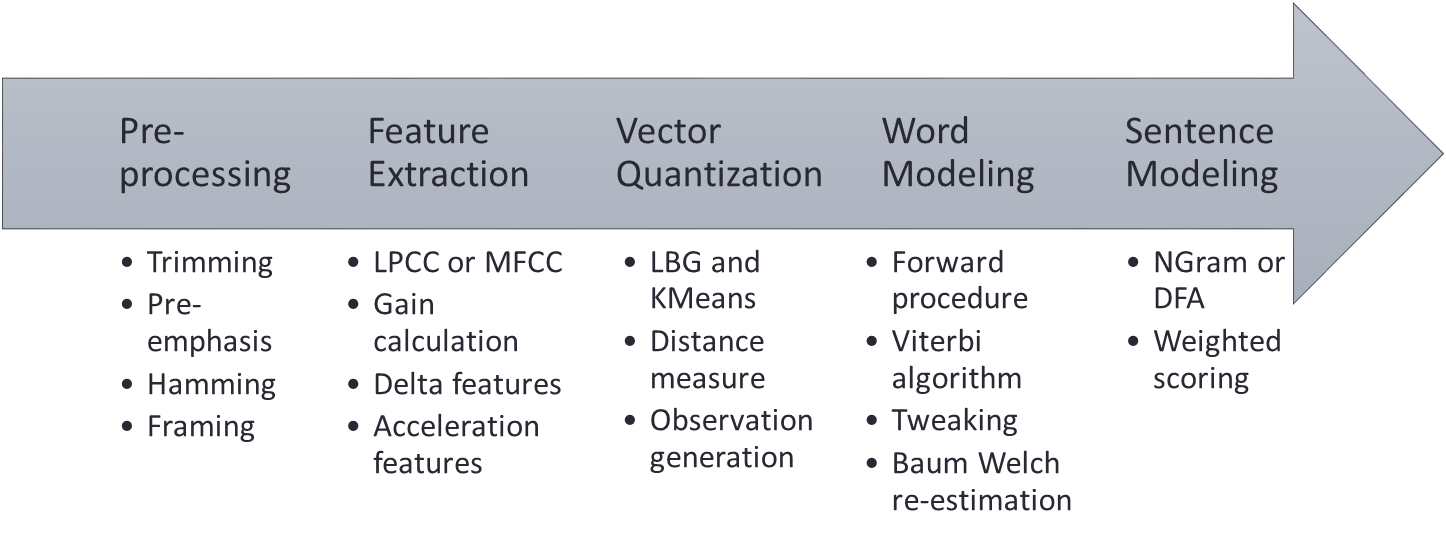
\includegraphics[scale=0.9]{training-flowchart}
    \label{fig:training-flowchart}
    \caption{Process flowchart}
\end{figure}

The appendix describes each of the stages of this process in good detail along with code implementation examples.

The library is written such that its clients do not have to dive deep into the technicalities of speech recognition. It has been divided into two abstraction layers:

\begin{enumerate}

\item Base

Provides implementation of various algorithms and techniques - Preprocessing, LPCC, MFCC, Derivative features, KMeans, LBG, HMM, NGram. Data objects - Codebook, Feature, Model, Gram are also described in this layer.

\begin{figure}[h!]
    \centering
    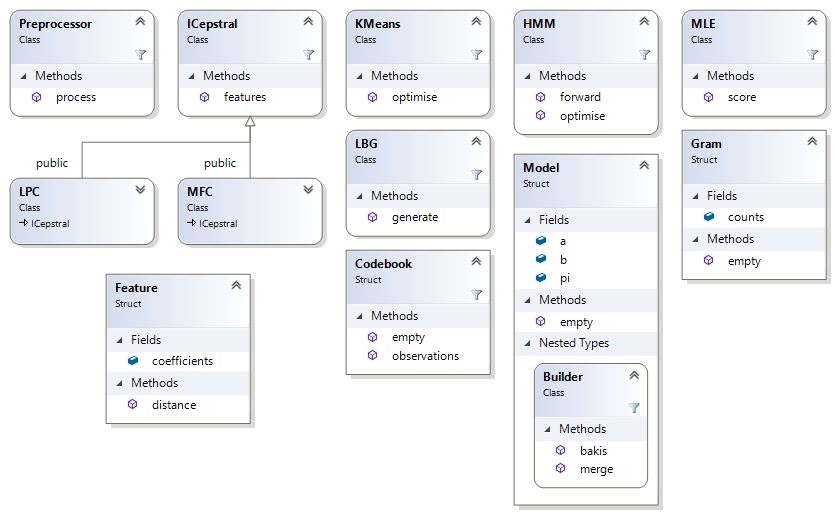
\includegraphics[scale=0.8]{sr-lib-base}
    \label{fig:sr-lib-base}
    \caption{Architecture of Base}
\end{figure}

Scaling has been done wherever necessary to avoid the floating point errors, and various optimizations have been made whenever possible. 

This layer is not parallelized and strictly does not interact with the input/output e.g. WAV audio or saving/loading the data objects to the file system.

\item Word

Provides training and testing interfaces. The clients of the library are only allowed to interact with this layer.
This layer foresees construction and testing of HMM and NGram models. It implements handling inputs - WAV audio files, word list, sentence list, etc. It also implements functions to save and read generated data objects to and from the file system.

\begin{figure}[h!]
    \centering
    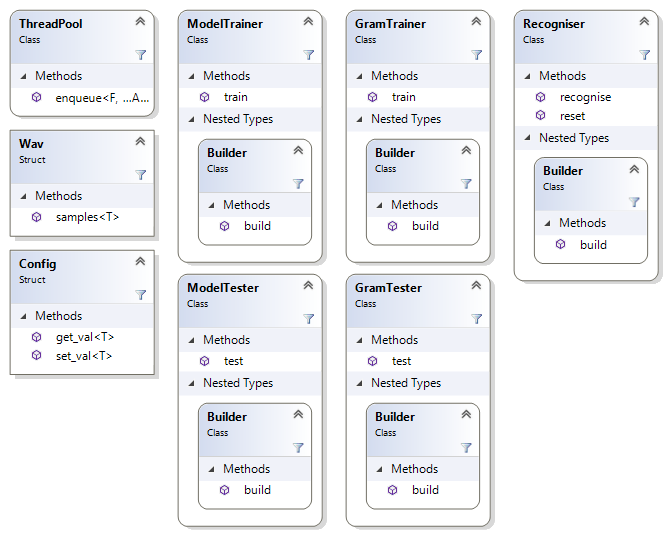
\includegraphics[scale=0.8]{sr-lib-word}
    \label{fig:sr-lib-word}
    \caption{Architecture of Word}
\end{figure}

This layer also handles the parallelization and configuration of the library.

The following tasks are parallelized:
\begin{itemize}
    \item Feature generation of multiple utterances
    \item Generation of multiple word models using HMM
    \item Matching of the input utterance with multiple word models
\end{itemize}

\begin{table}[h!]
    \centering
    \begin{tabular}{lll}
        Key          & Type &    Description \\ \hline
        q\_cache     & bool &    whether cached training files should be used \\
        n\_thread    & int &     number of threads used for parallel execution \\
        q\_trim      & bool &    whether the samples should be trimmed for background noise \\
        x\_frame     & int &     number of samples in a frame \\
        x\_overlap   & int &     number of samples to be overlapped while framing \\
        cepstra     & string &   mfc or lpc variants of feature generation \\
        n\_cepstra   & int &     number of features \\
        n\_predict   & int &     P of autocorrelation, only for lpc \\
        q\_gain      & bool &    whether gain term should be added to features \\
        q\_delta     & bool &    whether delta terms should be added to features \\
        q\_accel     & bool &    whether accel terms should be added to features \\
        x\_codebook  & int &     size of codebook \\
        n\_state     & int &     number of states in HMM \\
        n\_bakis     & int &     connectedness of initial bakis model for HMM \\
        n\_retrain   & int &     number of times each model should be trained \\
        n\_gram      & int &     number of previous words to be considered for prediction \\
        q\_dfa       & bool &    command based word prediction or probability based \\
        gram\_weight & double &  linear weight for the final scoring with recognition result \\
        cutoff\_score & double &  cutoff for final score \\
    \end{tabular}
    \caption{Keys for the configuration}
\end{table}

\end{enumerate}

As this is a word based recognition system, the basic unit of recognition in the library is a word. During the training, HMM Models are generated for each word, and the probabilities of occurrence of the words are calculated by parsing the sentence list. These probabilities are saved as NGram or DFA models depending upon the configuration.

During testing, a sentence is input as a combination of words.
For each word A in the sentence, and for each word B in the training data, following steps are taken:
\begin{itemize}
    \item Using HMM model of B find probability of occurrence of A.
    \item Using NGram models, find probability of occurrence of B given A's position in the input sentence.
    \item Final score is a linear combination of these two scores.
\end{itemize}
The word B with the maximum final score is best possible recognition. If its score is lesser than cutoff score, discard it, else output it.

\section{Graphical User Interface for Training}

The desktop graphical user interface is written in Swing Java framework. The interface can be run on Windows or Linux based OSes. It uses the Java Native Interface (JNI) for communicating with the speech recognition library.

\begin{figure}[h!]
    \centering
    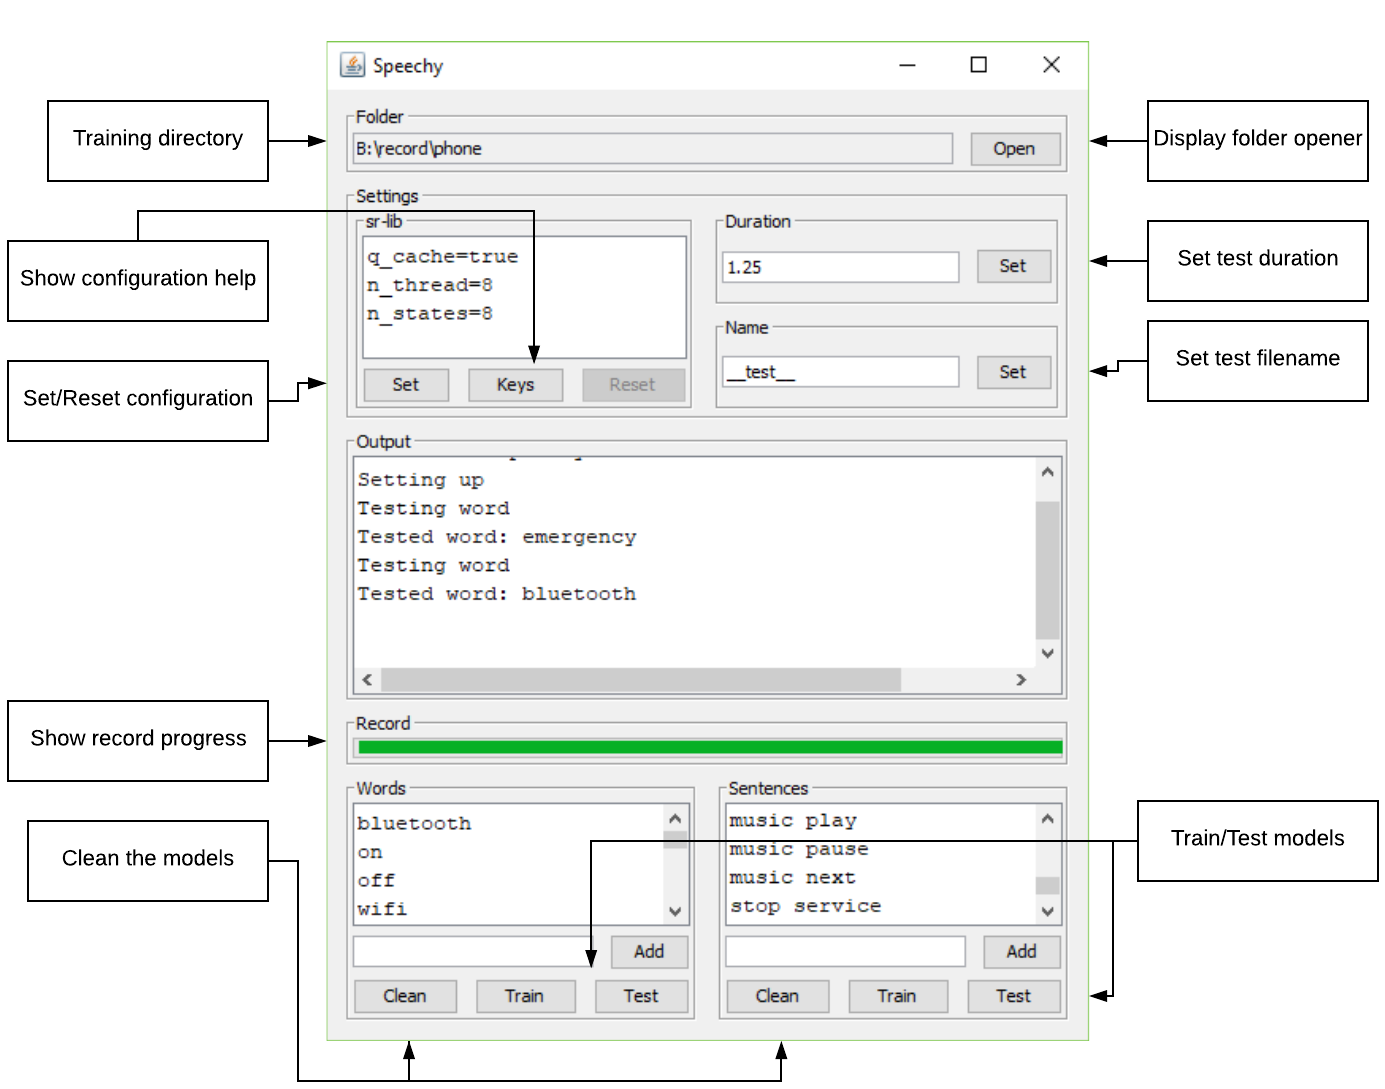
\includegraphics[scale=0.85]{desktop-screenshot}
    \label{fig:desktop-screenshot}
    \caption{Graphics User Interface for Training}
\end{figure}

\newpage

The interface has been made intuitive. Buttons are enabled only when required. For example, Test and Clean button will not be available until training is finished. At any moment only one task can be performed from the interface, and data race conditions between GUI and IO are avoided. The system is completely asynchronous and does not block the user interface.

\section{Voice Controlled Assistant for Android}

The android application is written in Kotlin and uses the Android NDK to run the speech recognition library.
The design of this application is inspired by Facebook Messenger chat heads. The main button is controlled by a service class that runs in the background. The main button is completely movable over the screen. It displays a round progress bar of the recording being done. A single click on the button starts recording for a sentence and user is expected to speak. A message toast is shown with every recognized word. If the recognition results match the list of actions, the corresponding action is performed. Currently, the application supports the following actions:
\begin{itemize}
    \item Open applications
    \item Enable/disable Bluetooth
    \item Control music player
    \item Enable/disable Wi-Fi
    \item Make phone calls
    \item Control brightness        
    \item Enable/disable torch
    \item Control volume
\end{itemize}

\begin{figure}[h!]
    \centering
    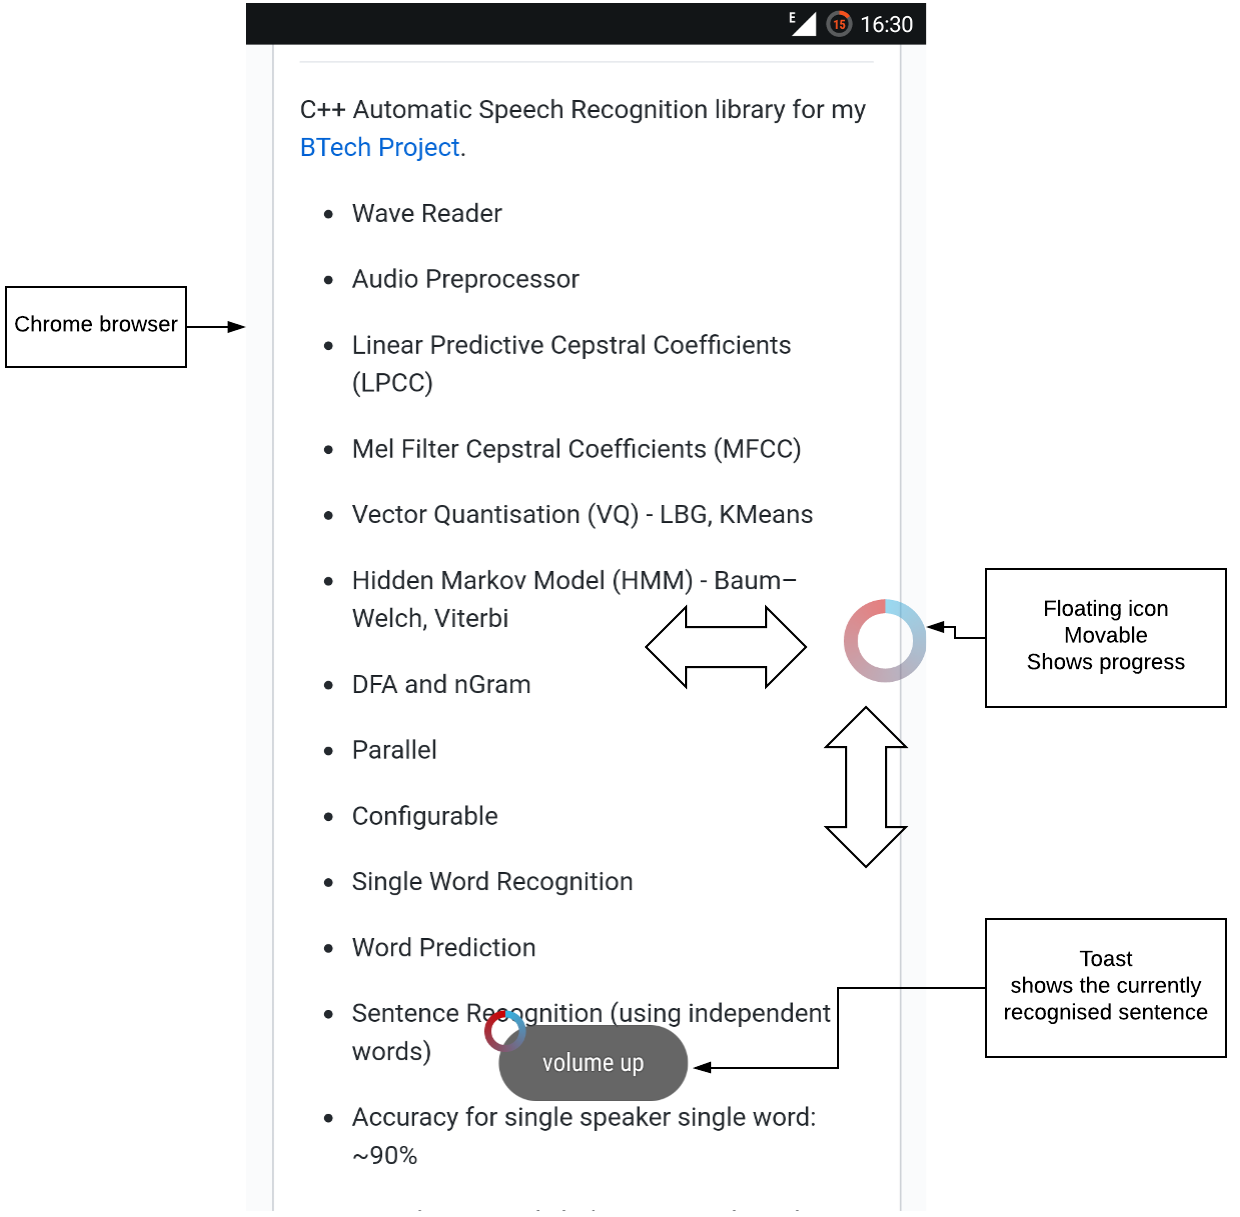
\includegraphics[scale=0.9]{android-screenshot}
    \label{fig:android-screenshot}
    \caption{Android Voice Controlled Assistant}
\end{figure}

The application makes extensive use of Kotlin’s co-routines to provide responsive GUI feedback. With the architecture of the application, more actions can be added with ease. To improve accuracy, the application also saves the recordings that are recognized so they can be trained by connecting to the desktop.
